\providecommand{\main}{..}
\documentclass[\main/main.tex]{subfiles}
\begin{document}

\section{Introduzione}

Si tratta di un argomento legato all'apprendimento non supervisionato, che si occupa di raggruppare oggetti simili tra loro.

\begin{definition}[Centroide]
  Il baricentro dei punti di un cluster è detto \textbf{centroide} (figura \ref{centroids}) ed ha caratteristiche identificative di quel cluster.
  \begin{figure}
    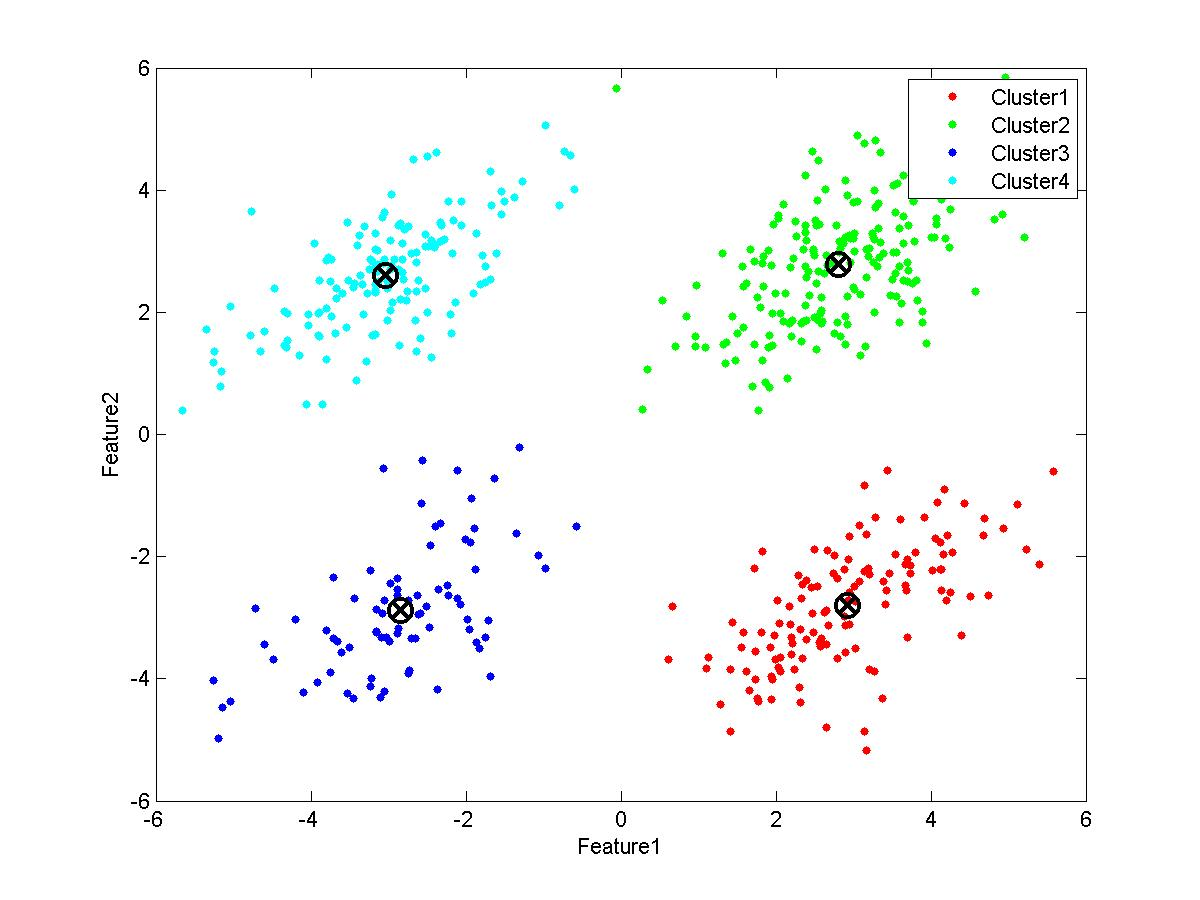
\includegraphics[width=0.5\textwidth]{centroid}
    \caption{Centroidi}
    \label{centroids}
  \end{figure}
\end{definition}

\begin{definition}[Clustroide]
  Un clustroide è un punto rappresentativo del cluster che non coincide con il \textbf{centroide}.
\end{definition}

\begin{figure}
  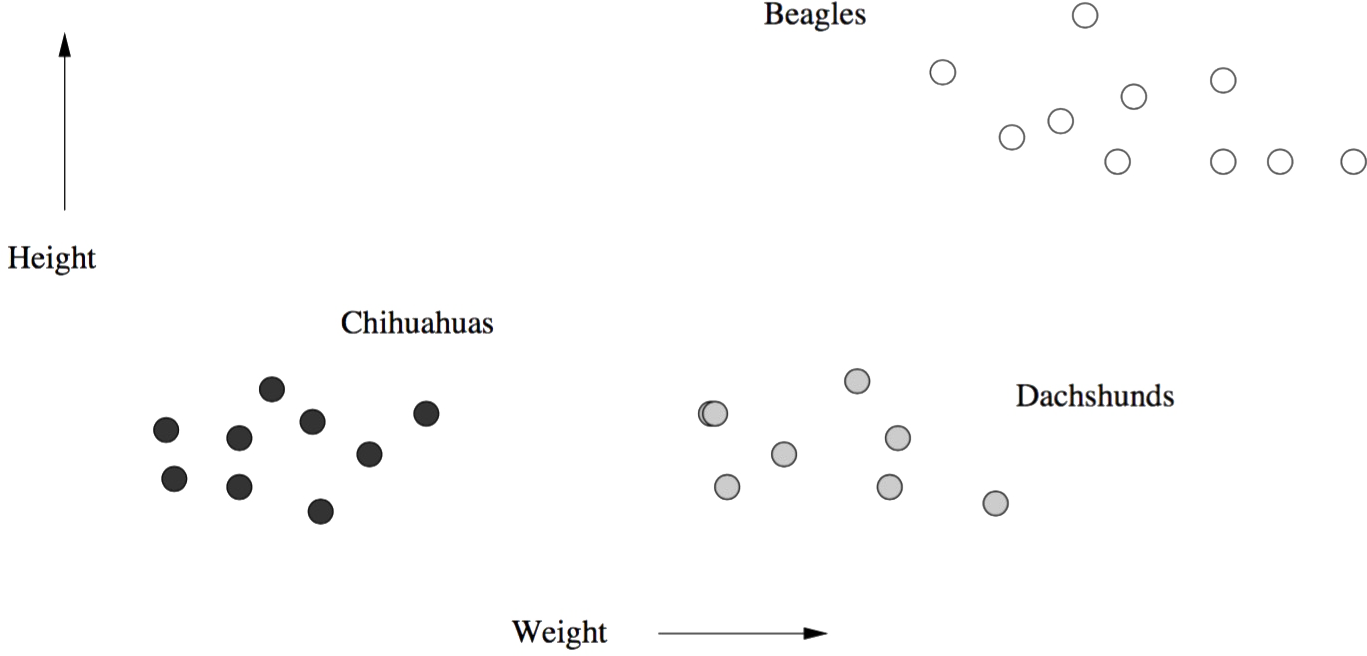
\includegraphics[width=0.75\textwidth]{dogs}
  \caption{Clustering di cani}
  \label{dog}
\end{figure}

\subsection{Esempio: clustering di cani}
Preso in considerazione per esempio uno spazio euclideo di 2 dimensioni, altezza e peso di alcuni cani. Viene considerato noto che le misurazioni siano solo di chihuhua, beagle e bassotti (Figura \ref{dog}).
Sicchè le zone sono ben identificate, potrebbe esserci una funzione tra altezza e peso, per esempio la razza del cane. Posso quindi dividere in 3 categorie, che posso utilizzare per classificare le razze di cane.

\section{The curse of dimensionality}
In uno spazio ad alta dimensione, la distanza euclidea tende a risultare costante. Inoltre, in uno spazio euclideo ad alta dimensione i vettori tendono ad essere normali tra loro.

\section{Approccio agglomerativo alla creazione di cluster}
Inizio costruendo un cluster per ogni punto e quindi procedo ad unire i cluster che io ritengo simili fra loro.

\begin{enumerate}
  \item Costruisco i cluster singoletti.
  \item while (!stop) $\{$
        \begin{enumerate}
          \item Scelgo due cluster
          \item Unisco i due cluster
        \end{enumerate}
  \item $\}$
\end{enumerate}

Una regola possibile per fondere due cluster è identificare i punti più vicini tra i due centroidi. Una volta fusi, si ridetermina il nuovo centroide.

\begin{enumerate}
  \item Scelgo due cluster vicini e li unisco.
  \item Ridetermino il centroide del nuovo cluster così ottenuto.
  \item Ripeto sino a che non determino che i custer sono sufficientemente grandi.
\end{enumerate}

Questo procedimento ha complessità $O(n^3)$.

\begin{figure}
  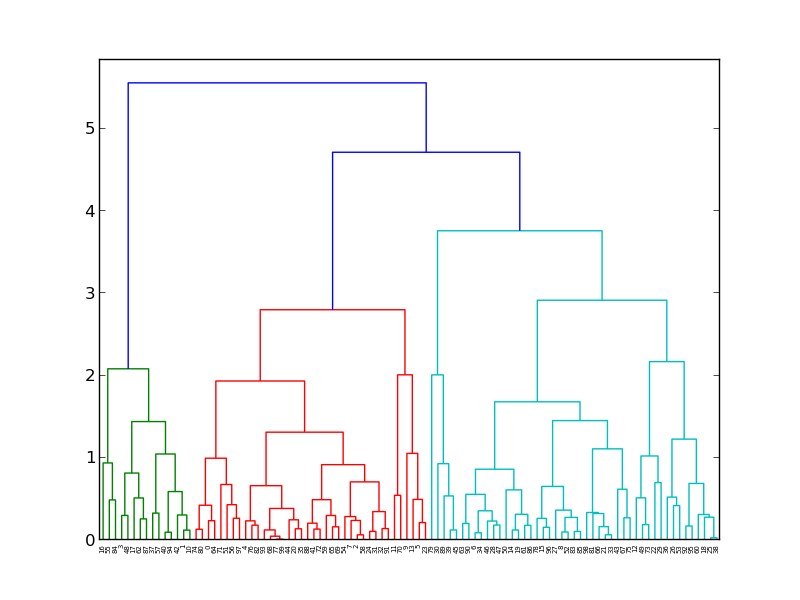
\includegraphics[width=0.5\textwidth]{dendrogram}
  \caption{Dendrogramma}
  \label{fig:dendrogram}
\end{figure}

\begin{definition}[Dendrogramma]
  Un dendrogramma (figura \ref{fig:dendrogram}) è un metodo grafico con cui rappresentare come i cluster si uniscono di iterazione in iterazione.
\end{definition}

\subsection{Approccio agglomerativo a complessità computazionale ridotta}

\begin{enumerate}
  \item Calcolo la distanza tra $n^2$ coppie \dotfill \textbf{$O(n^2)$}
  \item Costruisco una coda di priorità tra gli elementi simili \dotfill \textbf{$O(n^2)$}
  \item \underline{Elimino le coppie dei cluster che fondo} \dotfill \textbf{$O(n\log n)$}
  \item \underline{Inserisco nelle coppie il nuovo cluster} \dotfill \textbf{$O(n\log n)$}
\end{enumerate}

La sezione \underline{iterative}, sottolineata nella lista, viene ripetuta $n$ volte, quindi la complessità computazionale risulta essere $O(n^2\log n)$.

\subsection{Quando fermare l'algoritmo?}
L'algoritmo viene interrotto quando i cluster diventano troppo poco densi o il raggio del cluster troppo ampio (il raggio può essere calcolato sia dal centroide che dal clustroide).

\section{Algoritmi di clustering}

\subsection{K-Means}
Questo algoritmo per la creazione di cluster presuppone di lavorare in uno spazio euclideo. Preso un generico punto, vado ad identificare il centroide più vicino (che è sempre identificabile perché siamo in uno spazio euclideo per ipotesi) ed una volta identificato il cluster aggiungo ad esso il punto.

Il K in ``K-means'' indica il numero di cluster che io mi aspetto di trovare, numero che viene ipotizzato inizialmente.

\begin{enumerate}
  \item Fisso $k$ cluster ed identifico i loro centroidi.
  \item Per ogni punto:
        \begin{enumerate}
          \item Assegno il punto al centro più vicino.
          \item Ricalcolo il centroide.
        \end{enumerate}
\end{enumerate}

Posso o scegliere i cluster tramite un altro algoritmo oppure vado a scegliere $k$ punti, il più possibile distanti tra loro. Per questa seconda opzione si può:

\begin{enumerate}
  \item Scegliere un punto a caso
  \item Finché non si hanno selezionati $k$ punti
        \begin{enumerate}
          \item Aggiungi il punto che massimizza la sua distanza minima rispetto agli altri punti.
        \end{enumerate}
\end{enumerate}

\begin{figure}
  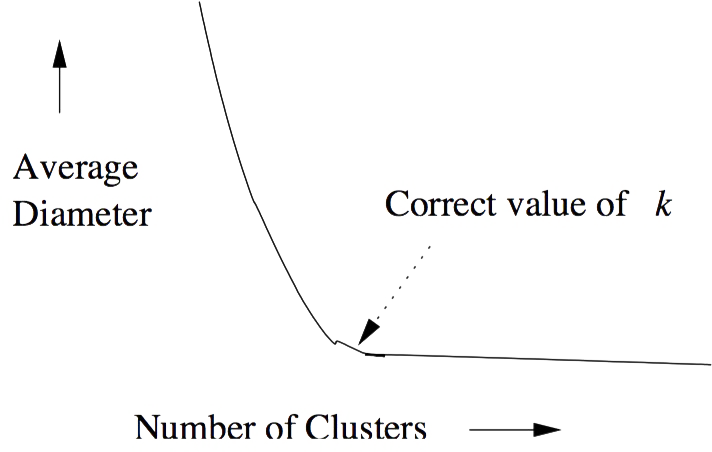
\includegraphics[width=0.5\textwidth]{raggio_K}
  \caption{Come il raggio varia in funzione di $k$}
  \label{fig:raggio}
\end{figure}

Per scegliere il numero $k$ di cluster posso andare a scegliere un numero e poi misurare con qualche fitness il risultato, per esempio il raggio \ref{fig:raggio} o la densità dei cluster. Una buona successione per scegliere il valore iniziale di $k$ è $2^n$, e poi una volta individuato un intervallo interessante perfezionare la scelta dicotomicamente.

\subsection{BFR}
Si tratta di un'estensione di k-means che non solo assume lo spazio euclideo ma anche che i punti seguano una distribuzione \textbf{normale multivariata}.

\subsubsection{Cosa  una normale multivariata?}
Prendiamo due variabili aleatorie, $X,Y \approx N(\mu, \sigma^2) \text{ con } X\bot Y$.

\begin{align}
  f_{X,Y} (x,y) & =                                                                                                                                     \\
                & =f_X (x) f_Y(y)                                                                                                                       \\
                & = \frac{1}{\sqrt{2 \pi \sigma^2}} e^{- \frac{(x-\mu)^2}{2\sigma^2}} \frac{1}{\sqrt{2 \pi \sigma^2}} e^{- \frac{(y-\mu)^2}{2\sigma^2}} \\
                & = \frac{1}{2 \pi \sigma^2} e^{-\frac{1}{2\sigma^2}[(x-\mu)^2+(y-\mu)^2]}
\end{align}

Se vado a cercare di identificare ora una curva di livello ponendo la funzione appena ricavata pari ad una costante $k$, posso semplificarla e ridurla ad un cerchio che ha come raggio $\sqrt{k}$ e centro $C = (\mu,\mu)$.

\[
  (x-\mu)^2 + (y-\mu)^2 = k
\]

Se le due variabili appartenessero invece a due distribuzioni differenti otterrei un ovale: $X \approx N(\mu_X, \sigma^2), Y \approx N(\mu_Y, \sigma^2) \text{ sempre con } X\bot Y$. Questa distribuzione combinata viene chiamata \textbf{normale bivariata}.


Nel caso io abbia $n$ variabili, invece, vado ad ottenere una \textbf{normale multivariata}, con la densità rappresentata in figura \ref{fig:multivariata}.

\begin{figure}
  \[
    \frac{1}{(\sqrt{2 \pi \sigma^2})^k} e^{- \frac{1}{2} \sum_{i=1}^k \frac{(x_i-\mu_i)^2}{\sigma_i^2}}
  \]
  \caption{Densità di distribuzione normale multivariata (caso con varianze $\sigma^2$ costanti)}
  \label{fig:multivariata}
\end{figure}

\subsubsection{Perché serve una normale multivariata?}
L'algoritmo richiede questa distribuzione perché va ad utilizzare la sua densità (o meglio, una sua versione semplificata) per scegliere a quale cluster aggiungere il punto. Ci interessa unicamente il coefficiente dell'esponenziale della distribuzione, che prende il nome di \textbf{distanza di Mahalanobis} (figura \ref{fig:Mahalanobis}).

\subsubsection{Distanza di Mahalanobis}
Se le distanze di Mahalanobis da un punto sono tutte molto grandi, il punto rimane in un ``limbo'', altrimenti esso viene assegnato al cluster più vicino.

\begin{figure}
  \begin{subfigure}{.5\textwidth}
    \[
      d(x,y) = \sqrt{\sum_{i=1}^d \left(\frac{x_i - y_i}{\sigma_i}\right)^2}
    \]
    \caption{Distanza di Mahalanobis}
    \label{fig:Mahalanobis}
  \end{subfigure}%
  \begin{subfigure}{.5\textwidth}
    \centering
    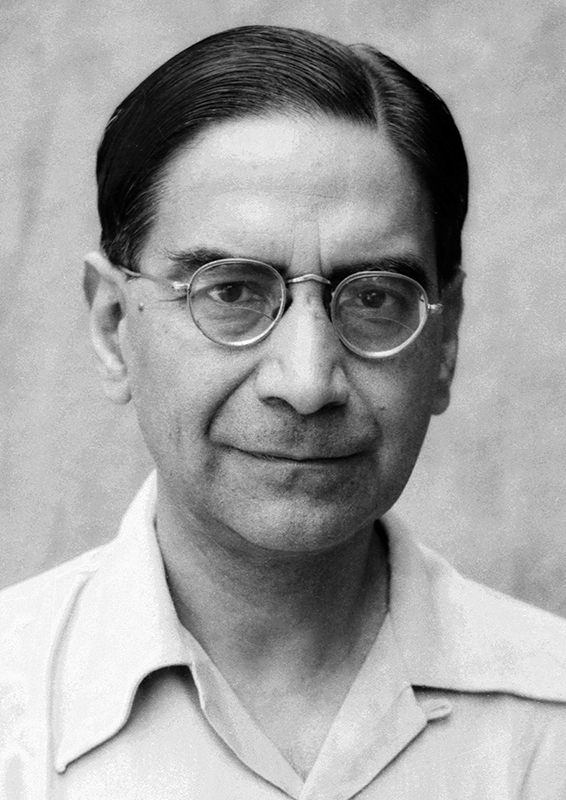
\includegraphics[width=.4\linewidth]{m}
    \caption{Prasanta Chandra Mahalanobis}
  \end{subfigure}
\end{figure}

\subsubsection{Il funzionamento}
Ad ogni dato momento esistono 3 set: il \textbf{compressed set} sei punti classificati, il \textbf{retain set} dei punti singoletto (il ``limbo'' a cui ci si riferiva prima) ed il \textbf{discard set} dei punti non classificati.

Ogni oggetti cluster ha i seguenti attributi:

\begin{enumerate}
  \item $N$: cardinalità dei punti nel cluster.
  \item \textbf{sum:} somma dei punti.
  \item \textbf{sumsq:} somma quadrata dei punti.
\end{enumerate}

Vengono usate somme e non moltiplicazioni per evitare la propagazione di eventuali errori di misura dei dati.

La varianza $\sigma^2$ viene calcolata, dati gli attributi sovra elencati, come:

\[
  \var(X) = E[X^2] - E[X]^2 \approx \sqrt{\frac{1}{N} \text{sumsq} - \left(\frac{1}{N} \text{sum}\right)^2}
\]

\begin{enumerate}
  \item Fisso un numero $k$ tramite una delle tecniche precedentemente elencate.
  \item Fisso $k$ cluster e determino per ognuno il centroide.
  \item Procedo su un chunk di punti (lo porto in memoria centrale) e li catalogo in uno dei set.
  \item Carico un nuovo chunk e ripeto.
  \item Ogni $n$ chunk elaboro i punti nel \textbf{retain set} e nel \textbf{discard set}, cercando di individuare nuovi cluster.
\end{enumerate}


\end{document}